\documentclass[twoside,twocolumn,8pt]{extarticle}
\usepackage{subfigure}

% ------
% Fonts and typesetting settings
\usepackage{amsmath}
\usepackage{amssymb}
\usepackage[sc]{mathpazo}
\usepackage[T1]{fontenc}
\linespread{1.05} % Palatino needs more space between lines
\usepackage{microtype}


% ------
% Page layout
\usepackage[hmarginratio=1:1,top=10mm,columnsep=20pt,left=0.8in, right=0.8in]{geometry}
\usepackage[font=it]{caption}
\usepackage{paralist}
\usepackage{multicol}

% ------
% Lettrines
\usepackage{lettrine}


% ------
% Abstract
\usepackage{abstract}
	\renewcommand{\abstractnamefont}{\normalfont\bfseries}
	\renewcommand{\abstracttextfont}{\normalfont\itshape}


% ------
% Titling (section/subsection)
\usepackage{titlesec}
\renewcommand\thesection{\Roman{section}}
\titleformat{\section}[block]{\large\scshape\centering}{\thesection.}{1em}{}

\usepackage{graphicx}
% ------
% Header/footer


\usepackage{fancyhdr}
\pagestyle{fancy}

\setlength\headheight{90.0pt}
\addtolength{\textheight}{-90.0pt}

\fancypagestyle{firststyle}
{
   	\fancyhead[L]{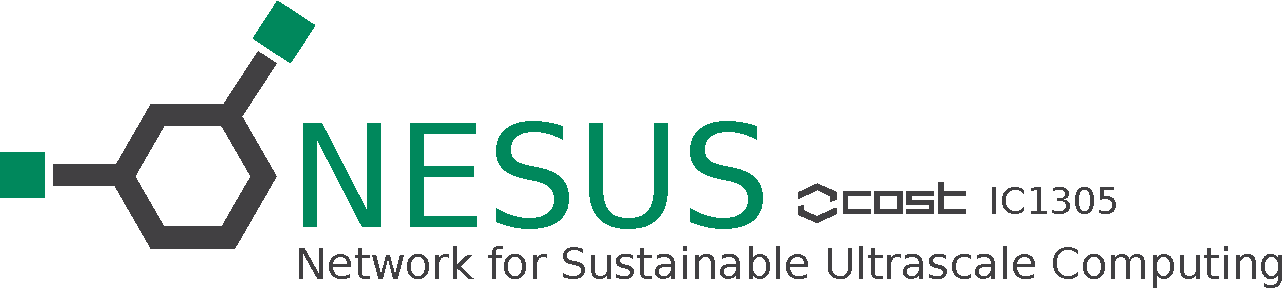
\includegraphics[height=5.5em]{pictures/nesus.pdf}}
	\fancyhead[C]{}
	\fancyfoot{}
	\fancyhead[R]{\small{Book paper template $\bullet$ October 2016 $\bullet$ Vol. I, No. 1}}
	\fancyfoot[RO,LE]{\thepage}
}
	\fancyhead[R]{}
	\fancyhead[L]{}
	\fancyfoot{}
	\fancyhead[C]{\small{Book paper template $\bullet$ October 2016 $\bullet$ Vol. I, No. 1}}
	\fancyfoot[RO,LE]{\thepage}


% ------
% Clickable URLs (optional)
\usepackage{hyperref}

% ------
% Maketitle metadata
\title{\vspace{-10mm}%
	\fontsize{24pt}{10pt}\selectfont
	\textbf{Automatic Cache Aware Roofline Model Building and Validation Using Topology Detection}
	}
	
		
\author{%
	\large
	\textsc{Nicolas Denoyelle \& Aleksandar Ilic \& Brice Goglin \& Leonel Sousa \& Emmanuel Jeannot} \\[2mm]
	\normalsize{	Inria - France -- INESC-ID -- Portugal}\\
	\normalsize{	\href{mailto:nicolas.denoyelle@inria.fr}{nicolas.denoyelle@inria.fr} \href{mailto:ilic@sips.inesc-id.pt}{ilic@sips.inesc-id.pt} \href{mailto:brice.goglin@inria.fr}{brice.goglin@inria.fr} \href{mailto:las@sips.inesc-id.pt}{las@sips.inesc-id.pt}} \href{mailto:emmanuel.jeannot@inria.fr}{emmanuel.jeannot@inria.fr}
	\vspace{-5mm}
	}

\date{}

\providecommand{\keywords}[1]{\textbf{\textit{Keywords}} #1}

%%%%%%%%%%%%%%%%%%%%%%%%
\begin{document}



\twocolumn[
  \begin{@twocolumnfalse}

\maketitle

\thispagestyle{firststyle}


\begin{abstract}
  \noindent The ever growing complexity of high performance computing systems imposes significant challenges to exploit as much as
  possible their computational and memory resources. Recently, the Cache-aware Roofline Model has gained popularity due to its
  simplicity when modeling multi-cores with complex memory hierarchy, characterizing applications bottlenecks, and quantifying
  achieved or remaining improvements. In this short paper we involve hardware locality topology detection to build  the
  Cache Aware Roofline Model for modern processors in an open-source locality-aware tool. The proposed tool also includes a set of
  specific micro-benchmarks to assess the micro-architecture performance upper-bounds.
  The experimental results show that by relying on the proposed tool, it was possible to  reach near-theoretical bounds of an Intel
  3770K processor, thus proving the effectiveness of the modeling methodology.
\end{abstract}


\keywords{Roofline Model, DRAM, Cache, Tool, Cache Aware Roofline Model, hwloc}

 \hrulefill
\bigskip 


\end{@twocolumnfalse}
]


\section{Introduction}\label{sec:Intro}
%+++++++++++++++++++++++++++
Since the advent of multi-core era, computer systems tend to incorporate an  increasing number of cores, while the relative memory
bandwidth and memory space per core is decreasing~\cite{MulticoreTrend}. In order to address application requirement and improve
the overall performance, current computing platforms rely on memory hierarchies of increasing complexity. Reshaping applications
data layout to take full advantage of those architectures can significantly improve the overall performance at the cost of
tremendous development efforts. The Cache Aware Roofline Model (CARM)~\cite{ilic2014cache} is able to aggregate this complexity in
a single insightful model, and guide application optimization to fit the micro-architecture performance upper-bounds. Its
effectiveness motivated us to bring it to non expert developer a robust tool equipped with deep benchmarking of multi-core
platforms with complex memory hierarchy, which automatically builds the model and provides the application optimization insights.\\

To  conduct a thorough evaluation of memory and compute capabilities of a given platform, the proposed tool also includes the
necessary software support to identify both micro-architecture instruction set and cache topology. The former can be found with
compiler support~\cite{CompilerSupport}, whereas the latter has only been mastered in a portable way by hwloc (hardware locality)
library~\cite{broquedis:inria-00429889}.
By relying on this run-time detection of compute and memory resources, the proposed tool automatically instantiates a set of
custom platform-specific micro-benchmarks for deep evaluation of platform capabilities, upon which the Cache-aware Roofline Model
is generated. Furthermore, the proposed tool also includes a lightweight library to provide access to the
hardware counters and extract, at runtime, the application features to be mapped in the model. To the best of our knowledge, there
are no existing cross-platform and open-source tools  that allow automating this process (i.e building the CARM and mapping
applications in it).\\

The remainder of this paper is organized as follow: 
Section~\ref{sec:state_of_art} describes the original Roofline Model and the Cache Aware Roofline Model.
Section~\ref{sec:contrib} details our tool features, design choices to model the cache hierarchy, and take full advantage of the
architecture, and provides preliminary results.
Section~\ref{sec:conclusion} concludes the paper.

\section{The Roofline Model Then and Now}\label{sec:state_of_art}
%+++++++++++++

The Roofline modeling, in general, is an insightful approach to represent the performance upper-bounds of a processor
micro-architecture. Since computations and memory transfers can be simultaneously performed, the Roofline modeling is based on the
assumption that the overall execution time can be limited either by the time to perform computations or by the time to transfer
data. Hence, from the micro-architecture perspective, the overall performance (typically expressed in flops/s) can be limited by
the peak performance of computational units or by the capabilities of memory system (i.e., memory bandwidth). To this date, there
are two main approaches for Roofline modeling, namely: the Original Roofline Model (ORM)~\cite{Williams:2009:RIV:1498765.1498785}
and the Cache-aware~Roofline~Model~(CARM)~\cite{ilic2014cache}.
These two approaches provide different perspectives when describing the micro-architecture upper-bounds, and they are also
differently constructed, validated, and used for application characterization and optimization.

The ORM targets the systems with a processing element (PE) connected to a single (slow) memory (usually, the DRAM). The ORM's
PE encapsulates computational units and a set of fast memories (i.e., caches). As such, the ORM mainly considers the memory
transfers between the last level cache and the DRAM (commonly referred as DRAMBytes). Hence, it denotes the theoretical DRAM
bandwidth as one of the potential execution bottlenecks. Depending on the "operational intensity", i.e., the ratio of compute
operations (flops) over the quantity of DRAM data (DRAMBytes), the applications can be characterized as compute-bound or
memory-bound. The model was used in several works for application
optimization~\cite{Kim20111201}~\cite{Rossinelli2164}~\cite{vanNieuwpoort:2009:UMH:1542275.1542337}, as well as to model other.\\
%% We represented on the chart~\ref{fig:roofline_chart},
%% where the "operational intensity" stands on abscissa and the performance stands in ordinate.
%% The figure~\ref{fig:roofline_chart} shows that upon data layout optimization the performance and arithmetic intensity vary to hit
%% one of the mentioned elements' roof.

%% \begin{figure*}
%% \begin{center}
%%   \begin{minipage}[b]{0.49\textwidth}
%%     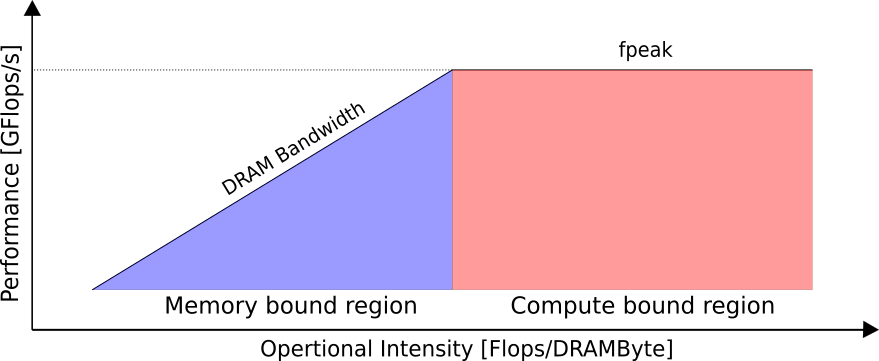
\includegraphics[width=\textwidth]{pictures/roofline_chart}
%%     \caption{ORM chart}
%%     \label{fig:roofline_chart}
%%   \end{minipage}
%%   \hfill
%%   \begin{minipage}[b]{0.49\textwidth}
%%     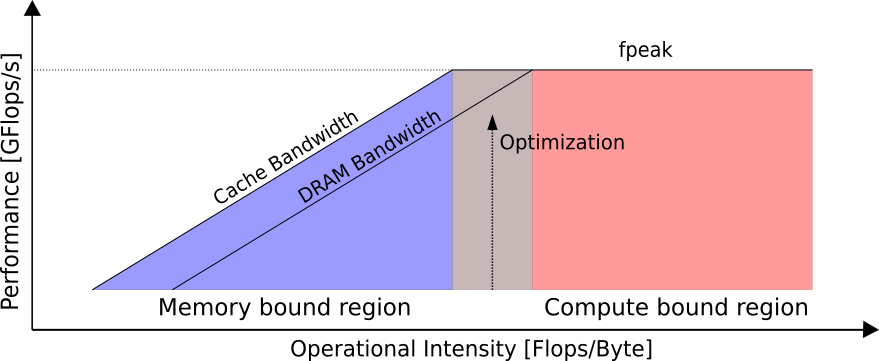
\includegraphics[width=\textwidth]{pictures/CARM_chart}
%%     \caption{CARM chart}
%%     \label{fig:CARM_chart}
%%   \end{minipage}
%%   \end{center}
%% \end{figure*}

In contrast, the CARM perceives the memory transfers from a consistent micro-architecture point of view, i.e., a core, where
the memory transactions are issued. As such, the CARM targets contemporary systems where the PE encloses only compute units
and registers, while all other memory levels are separately and explicitly considered. For this purpose, the CARM includes several
memory lines in the same plot, each corresponding to the realistically achievable bandwidth of a specific memory level to the core,
i.e., cache levels and DRAM. When characterizing the applications, the CARM relies on the true "arithmetic intensity", i.e., the
ratio of performed compute operations (flops) over the total volume of requested data (in bytes) by taking into account the
complete memory hierarchy (i.e., caches and DRAM).\\
%% This model is plot on chart ~\ref{fig:CARM_chart} and shows whether an
%% application with a given arithmetic intensity is memory-bound or compute-bound if a straight vertical line hit a peak (FP) roof
%% or a bandwidth roof.

For these reasons, we base our methodology on the Cache Aware Roofline Model. 
As explained above, the CARM differs from the original model, it is usually capable of providing deeper insights when analyzing the
applications execution bottlenecks, and it also has potential to be adapted to future memory designs. Moreover, the ORM has already
a dedicated tool~\cite{Lo2015} for a similar purpose as ours, but the approach adopted in the herein proposed tool significantly
differs and it targets a more consistent and concrete analysis.

\section{Locality-Aware Roofline Tool}\label{sec:contrib}
%+++++++++++++

Our main contribution consists in the development of the open-source tool named Locality Aware Roofline Tool (LART)\footnote{available at: https://github.com/NicolasDenoyelle/LARM-Locality-Aware-Roofline-Model-}, which
exploits hwloc topology detection to automatically build the Cache Aware Roofline Model (CARM).

\paragraph*{Main tool features.}

The proposed LART is composed of 3 main components, namely:
\begin{itemize}
\item A set of micro-benchmarks for automatic CARM construction on a given micro-architecture;
\item The library for counter-based extraction  of CARM metrics from a user application (i.e., the number of performed flops and
  transferred bytes, as well as the overall execution time);
\item A visualization tool to present the model with architecture bounds and applications metrics extraction.
\end{itemize}

The first component consists in a program that automatically  builds the CARM for the specific processor micro-architecture where
the tool is run. By relying on a set of hwloc features, the proposed tool automatically detects the memory hierarchy and processor
compute capabilities, based on which specific micro-benchmarks are instantiated to deeply evaluate the bandwidth of each memory
level,  as well as the peak floating point (FP) performance according to the CARM methodology.
In addition, the proposed tools also permits to perform the CARM validation tests, by running a set of micro-benchmarks with
variable arithmetic intensity. 
The second component of the tool represents  a library with a set of API calls. These API calls are aimed at performing the
automatic CARM characterization of a given user application, by instrumenting the application source code.
To provide a wider cross-platform portability, this component relies on PAPI~\cite{mucci1999papi} features to collect all
necessary CARM metrics via hardware performance counters, i.e., to determine the application arithmetic intensity and performance.
The third component of the proposed tool is a command-line generating a visual plot of the CARM using platform analysis results. It
enables a user to plot applications metrics extracted with the above-referred library in the CARM chart.
The model validation and bandwidth deviation can also be seen and provide a straightforward evaluation of the confidence one can
grant to the model.

\paragraph*{Building the model from a hierarchical topology}

\begin{figure}
  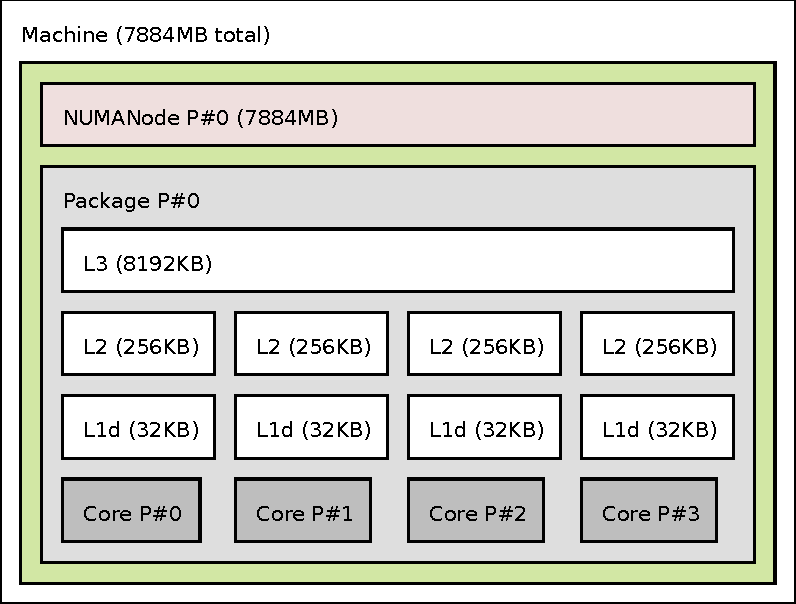
\includegraphics[width=.5\textwidth]{pictures/i7_3770k.pdf}
  \caption{Topology of Intel Ivy Bridge processor model i7 3770k as seen by hwloc}
  \label{fig:topology_adriana}
\end{figure}

Discovering all the computing and memory resources in a computing platform can be performed with tools such as
hwloc~\cite{goglin:hal-01330194}. Prior to hwloc,  the similar approaches were often less portable or they were not capable of
exposing as many details about cache sharing etc. The hwloc framework models the machine topology as a tree and suits particularly
well the caches structure.
As presented in Figure~\ref{fig:topology_adriana}, the view returned by the hwloc represents, express this structure with nested
boxes. Each core has a stack of 2 private caches, while all cores share the last level cache and the main memory (DRAM).
This model where each Core sees  the cache hierarchy as a cache stack of increasing size\footnote{
  The processors use a cache replacement policy where old data from closer caches is evicted in favor of more frequently used ones.
  The replacement policy defines the method how data is moved from bottom caches to top ones(see in
  Figure~\ref{fog:topology_adriana}). Since the size of the caches closer to cores is smaller than the one for the farther memory
  levels, the cache stack as seen by each core has an increasing size from bottom to top.
}, perfectly suits the way how the CARM perceives the memory hierarchy.
In addition, the hwloc library also allows a straightforward identification of the cache and memory sizes via the  attributes of
the Core parent nodes. These parameters are further used in the proposed tool  in order to instantiate the appropriate
micro-benchmarks for different memory subsystem levels by using the state of the art technique (i.e. buffer streaming of
increasing sizes).

\paragraph*{Reaching the architecture upper-bounds}

Nowadays, general purpose processors usually implement a variety of vector operations, also named as Single Instruction Multiple
Data (SIMD) operations. Depending on the target micro-architecture,  the tool proposed herein is able to automatically detect the
operation type that allows to fully exploit the micro-architecture capabilities  (typically, the widest vector instructions). These
instructions refer to both compute operations and memory transactions, where the performance upper-bound of each involved unit is
expressed as a function of the register size (i.e the number of floating point  elements it contains) and the achievable
throughput. By compiling the benchmarks on target architecture, we ensure that the largest vector size is used for the benchmarks
by interpreting the compiler macros. 

It is worth to emphasize that typically there are several types of memory/compute instructions on modern processors, and separate
hardware units capable of performing different operations simultaneously. For instance, a core
may perform a multiplication (MUL) and an addition (ADD) on separate FPUs, which  can also be performed in parallel when there are
no  dependencies between them. Hence, a core can provide significantly higher  performance for the codes that fully interleave ADD
and MUL operations. This principle also applies to the memory subsystem, where several ports can be dedicated in modern processors
to simultaneously serve different number of load (LD) and store (ST) operations, e.g., two LD and one ST 128-bit ports in the Intel
Ivy Bridge micro-architecture. Hence, in order to exercise the full  compute and memory capabilities of the target architecture,
the proposed tool relies on several types of operations to benchmark the platform and it selects by default the one used by
the CARM, e.g.for the Intel Ivy Bridge, it interleaves 2 LD and 1 ST instruction  when assessing the peak memory bandwidth, while
one ADD and one MUL are interleaved for peak FP performance. 

\paragraph*{LART Reproducing CARM Experimental Results on Intel Ivy Bridge}
\begin{figure*}
  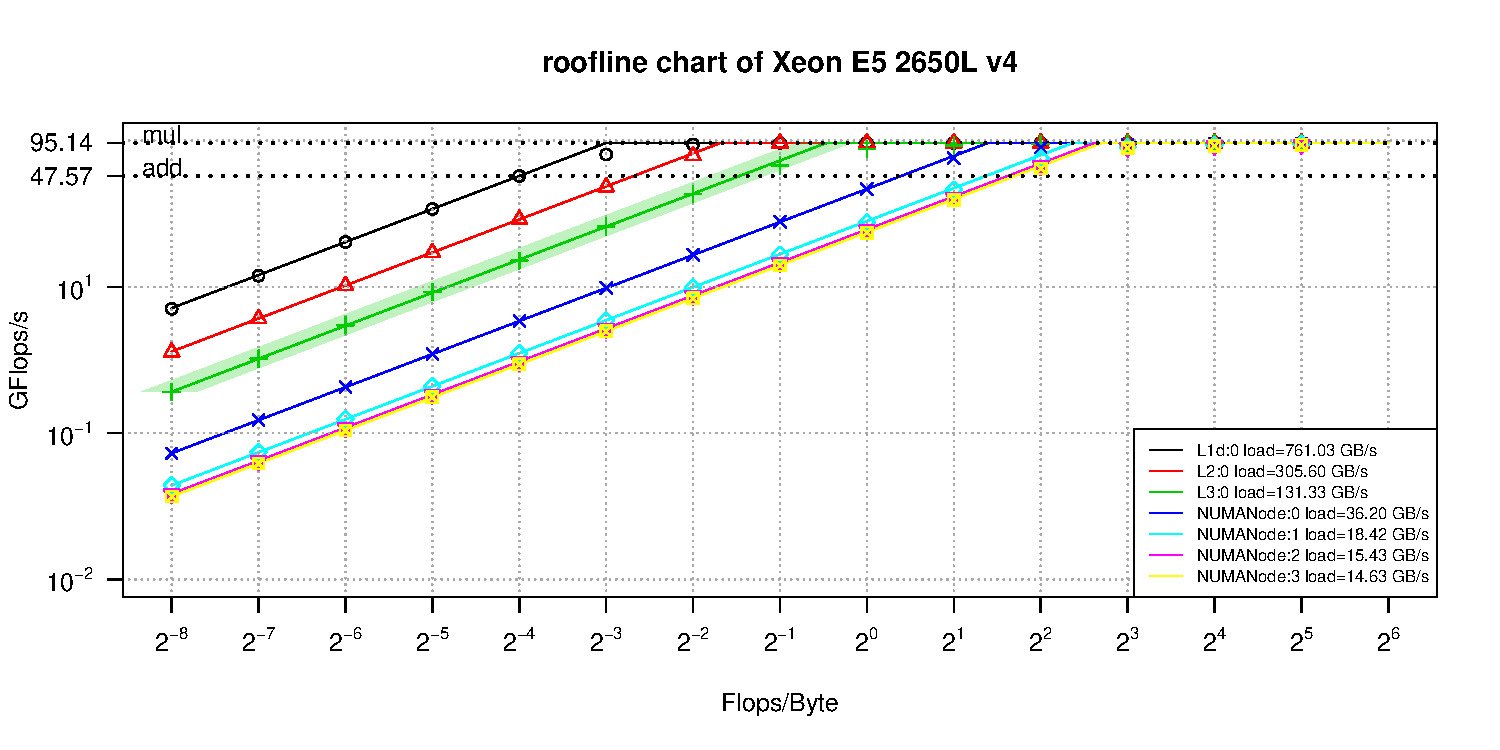
\includegraphics[width=\textwidth]{pictures/roofline_model}
  \caption{CARM on i7 3770k with LART tool.}
  \label{fig:LART_adriana}
\end{figure*}

Figure~\ref{fig:LART_adriana}, shows an output of the CARM plot generated by the herein proposed tool for an Intel i7
3770k (Ivy Bridge) processor, which topology is previously displayed in Figure~\ref{fig:topology_adriana}.
The black, red, green and blue oblique lines distinguish several regions of the attainable performance upper-bounds for AVX
instructions, which are limited by the bandwidth of different memory levels , i.e., L1, L2, L3 and DRAM, respectively.
The two horizontal lines represent the peak FP performance for MUL/ADD and multiplication with addition (MAD). 

It is worth to note that the proposed tool was capable of reaching the near-theoretical upper-bounds of the tested
micro-architecture both for the the L1 bandwidth and peak FP performance.  In particular, by relying on the CARM testing
methodology,  the throughput of 1.49 instructions per cycle (IPC) was achieved for the  L1 AVX-256 accesses. In addition, the
IPC of 1.98 was achieved for FP performance, which closely match the theoretical throughput of AVX FP instructions when overlapping
ADD and MUL operations.

The colored points matching the CARM lines represent the results of the validation benchmarks provided within the proposed tool,
i.e., a set of synthetic benchmarks tailored to hit the performance upper-bounds of the micro-architecture for different
arithmetic intensities.

As presented in Figure~\ref{fig:LART_adriana}, legend in the bottom right corner, includes first the memory subsystem,
then the micro-operation type(i.e. 2ld1st - interleaving of 2 LD and 1 ST) and the experimentally obtained bandwidth.
On the top right corner in Figure~\ref{fig:LART_adriana}, the legend refers to the tested applications for which the CARM metrics
were extracted with our library. Those applications express different arithmetic intensity and are well suited to be analyzed with
this model. In particular they represent application potential hot spot and come from well
known benchmarks named as HPCCG(from Mantevo~\cite{barrett2015assessing} mini-applications) and STREAM~\cite{mccalpin1995stream}.
Although deep performance evaluation of those applications is out of the scope of the
paper, it is worth to note that the proposed LART tool is capable of providing the facilities visually analyze the behaviour even
for real-world applications.

\section{Conclusion and future work}\label{sec:conclusion}
%+++++++++++++++++++++++++++++++++++

On the path of extreme scale computing, computer systems complexity is increasing to address hardware and software constraints.
The CARM is able to aggregate this complexity and by relying on hwloc topology detection capability we developped a robust tool to
build this model and characterize applications. The LART tool is capable of performing deep platform analysis,
as well as model validation with automatic detection of micro architecture capabilities and topology.
In order to further ease the burden of platform-specific benchmarking for non expert developers the proposed tool also provides a
library to project and visualize applications in the model.
The efficiency of the proposed tool was verified on a computing platform with Intel Ivy Bridge micro-architecture, where the
obtained experimental results show that the proposed tool was capable of reaching near-theoretical performance.

In a close future, we plan to extend the tool and the model to cover heterogeneous memory systems and show their usefulness to
improve data spatial locality in Non-uniform memory access (NUMA) systems, while the current model is manly used to improve data
temporal locality with cache usage optimization.

\bibliographystyle{plain}
\bibliography{references}

\end{document}
